\section{Introduction}
\label{sec:intro}
Opinion summarization aims at
producing a summary for a set of 
subjective user reviews about an entity (i.e.,
a product, a service or a movie), which can help users quickly understand the entity.
Opinion summarization is a specialized multi-document 
summarization~\cite{FabbriLSLR19,LiuSPGSKS18,multisumSIG21}.
Unlike traditional multi-document summarization, opinion summarization focuses on the aspects and opinions of entities in the input documents.
Deep learning techniques have made great successes 
in summarization~\cite{SeeLM17,LiuLZ18,BART20,liu2021keyword},
%\JQ{no relationship between although and later sentences} %\YZ{add our papers}, 
which require training on a large number of document-summary pairs.
Unfortunately, opinion summarization generally lacks the training pairs with reviews as input 
and summary as output, as it is difficult and costly for annotators to write 
summaries for multiple reviews (known as \textit{multi-reviews} in this paper) 
on a large scale.

\begin{table}[th]
	\centering
	\scriptsize
	\begin{tabular}{|m{7.2cm}<{\centering}|}
		\hline 
		\bf Synthetic Summary (sampled from the reviews)\\
		\hline
		\makecell[l]{very \textbf{disappointed} in \textbf{food} and \textbf{service} . the \textbf{beef} was \textbf{burned} . \\ 
			\textit{the \textbf{staff} \textbf{dismissed} my comments . }} 
		\vspace{0.2em}\\
		\hline
	\end{tabular}
	\begin{tabular}{|l|c|p{5cm}|}
		\hline
		\multicolumn{3}{|c|}{\bf Synthetic Input (to be summarized)}  \\	
		\hline
		\multicolumn{3}{|l|}{\bf Textual (unstructured)} \\
		\hline
		\multirow{3}{*}{\em Random} & $R_1$ & very average spanish \textbf{food} .
		\\
		%\cline{2-3}
		& $R_2$ &definitely not a peruvian restaurant
		.
		\\
		%\cline{2-3}
		& $R_3$ &love this place! location is great
		.
		\\ 
		\hline
		\multirow{3}{*}{\em Similarity} & $R_1$ & bad \textbf{food} and \textbf{service} . \textbf{disappointed} \\
		%\cline{2-3}
		& $R_2$& the \textbf{food} and \textbf{service} was not good . very \textbf{bad experience} .
		\\
		%\cline{2-3}
		& $R_3$ &awful \textbf{food} and \textbf{service} . the \textbf{staff} was unfriendly .
		\\
		\hline
		\multicolumn{3}{|l|}{\bf Structured} \\
		\hline
		OpiDig& OA & \textbf{disappointed}, \textbf{food; disappointed}, \textbf{service; burned}, \textbf{beef}
		\\
		\hline
		\multicolumn{3}{|l|}{\bf Mix-structured}  \\	
		\hline
		\multirow{3}{*}{\em Ours} &OA &not good, \textbf{food;} great, location\textbf{;} bad, \textbf{food; disappointed}, \textbf{service;} not fresh, \textbf{beef;} unfriendly, \textbf{staff;} awful, \textbf{service}\\
		%\hline
		&IS &not recommended .\textbf{;} my questions were \textbf{dismissed} .\textbf{;} the \textbf{staff} ignored our \textbf{comments} .\\
		\hline
	\end{tabular}
	\caption{A summary and various inputs synthesized by different methods. Matched words in both input and output are bolded.
		$R$ denotes textual review. 
		OA indicates explicit opinion-aspect pairs.
		The italicized sentence doesn't contain explicit OAs, 
		which is called ``implicit sentence'' (IS).
		``;'' delimits OAs and ISs. 
	}\label{tab:previous_data}  
\end{table}

In view of the above challenge, some approaches~\cite{MeanSum19,Copycat20,tree21}
adopt unsupervised learning, e.g., by using the auto-encoders.
They reconstruct individual reviews by encoding themselves
at training time, which may prevent them from effectively generating summary by 
encoding multi-review at test time. 
%\KZ{Why? Is it because at training time,
%they encode only a single review at a time?}
%Because the multi-review, including much redundant information, 
%is actually the noisy version of summary.
Other more popular approaches~\cite{Denoise20,Fewshot20,Plansum20,transsum21} 
focus on creating synthetic (multi-review, summary) pairs for training.
They typically sample one or more reviews from all reviews 
about an entity
as the ``pseudo'' summary, that is, the output of the synthetic training pair.
These approaches differ from each other by how the input is created.
Existing approaches use either {\em textual} or  {\em structured} information (see \tabref{tab:previous_data})
to create the input.

%\begin{figure}[th]
%	\centering
%	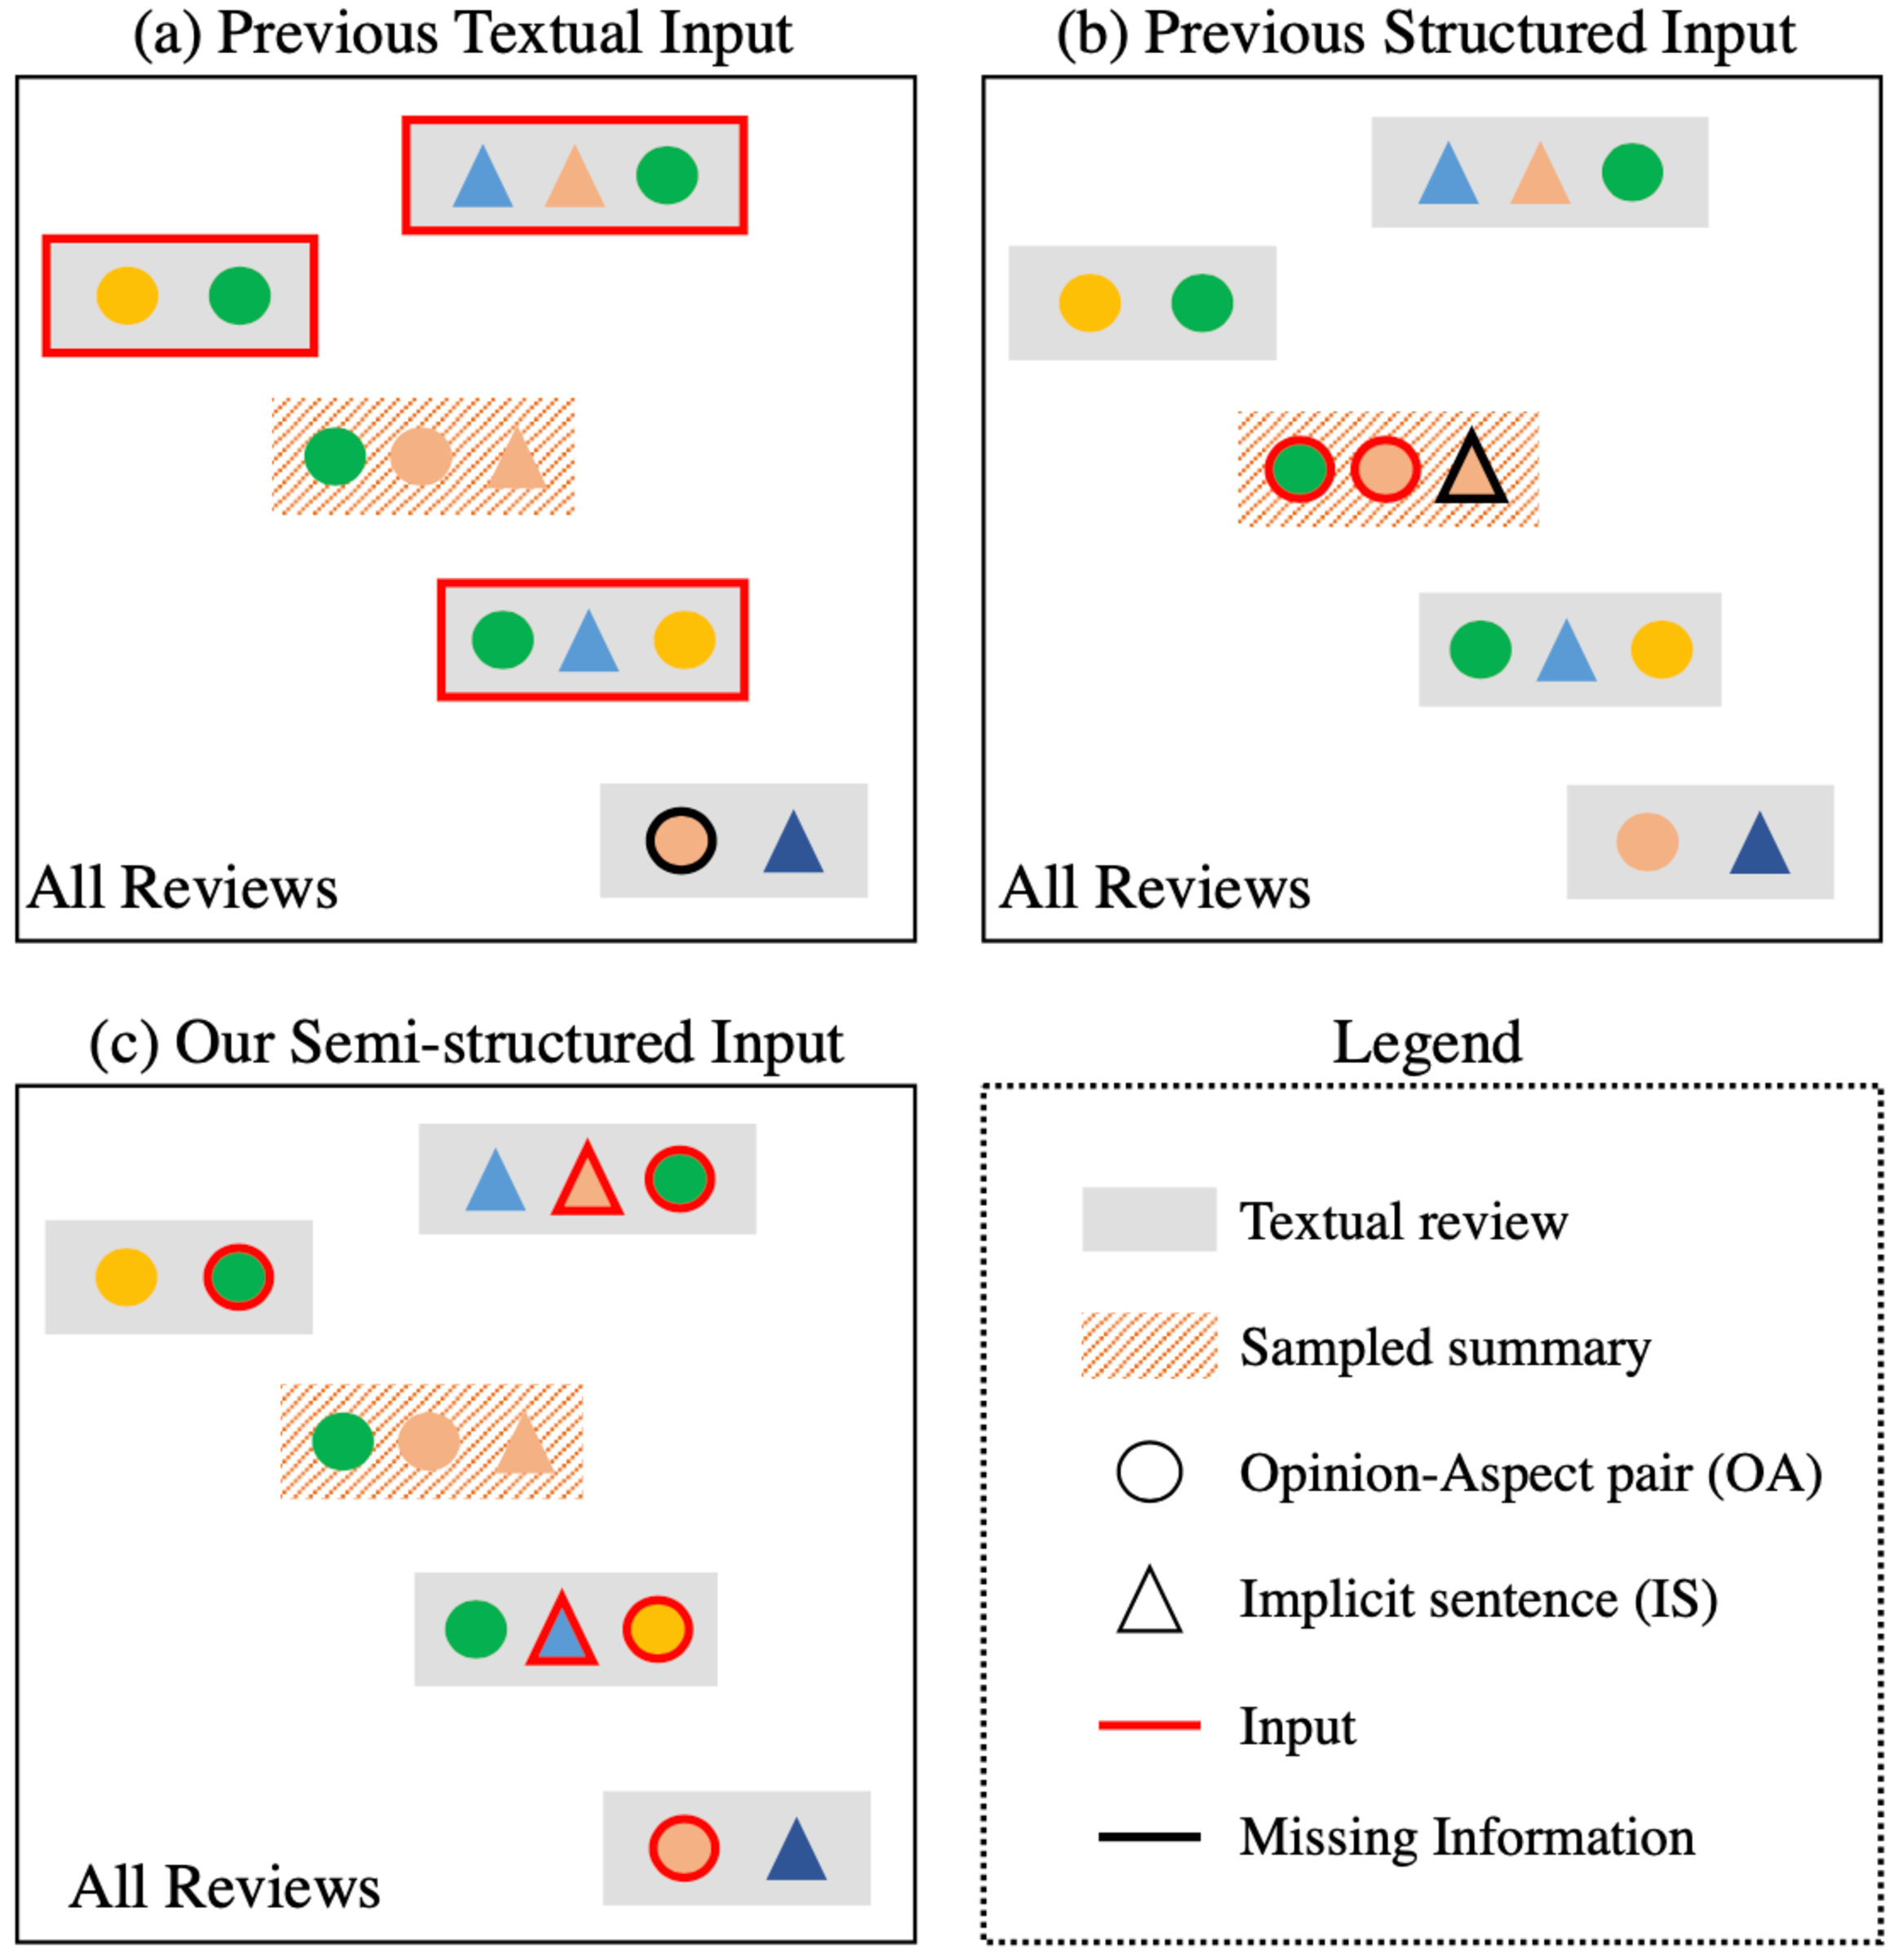
\includegraphics[width=0.85\linewidth]{./brief.pdf}
%	\caption{Different synthetic inputs of the same summary.
%	}
%	\label{fig:brief}
%\end{figure}
\cut{%%%%%%
\begin{table}[th]
	\centering
	\small
    \subtable[Output (sampled summary) with its OAs and ISs]{
	\begin{tabular}{|m{0.3cm}<{\centering}|p{7.1cm}|}
		\hline 
		%\rule{0pt}{10pt}
		\multicolumn{2}{|c|}{\rule{0pt}{10pt} \bf Output} \\
		\hline
		S & \makecell[l]{very \textbf{disappointed} in \textbf{food} and \textbf{service} . the \textbf{beef} was \\ \textbf{burned} . 
				\underline{the \textbf{staff} \textbf{dismissed} my comments .} } 
		\vspace{0.2em}\\
		\hline
		OA & \textbf{disappointed}, \textbf{food; disappointed}, \textbf{service; burned}, \textbf{beef} \\
		\hline
		IS   & the \textbf{staff} \textbf{dismissed} my comments . \\
		\hline
	\end{tabular}
}
\qquad
\subtable[Synthetic input based on summary in (a)]{
	\begin{tabular}{|m{0.9cm}|m{0.3cm}<{\centering}|m{5.8cm}|}
		\hline
		\multicolumn{3}{|c|}{\rule{0pt}{10pt} \bf Input}  \\	
		\hline
		\multicolumn{3}{|l|}{\bf Textual} \\
		\hline
		\multirow{3}{0.1cm}{FewSum} & $R_1$ & very average spanish \textbf{food} .
		\\
		\cline{2-3}
		& $R_2$ &definitely not a peruvian restaurant
		.
		\\
		\cline{2-3}
		& $R_3$ &love this place! location is great
		.
		\\
		\hline
		\multirow{3}{0.1cm}{Denoise} & $R_1$ & very uncomfortable in \textbf{food} and \textbf{staff} . the \textbf{ food} was bad . the \textbf{staff} ignored me .
		\\
		\cline{2-3}
		& $R_2$ & bad \textbf{food} . the \textbf{staff} ignored me . very uncomfortable in restaurant .\\
		\cline{2-3}
		& $R_3$ &I was \textbf{disappointed} with the restaurant. the \textbf{food} was not bad . but the \textbf{staff} was unfriendly .
		\\
		\hline
		\multirow{3}{0.1cm}{PlanSum} & $R_1$ & bad \textbf{food} and \textbf{service} . \textbf{disappointed} \\
		\cline{2-3}
		& $R_2$& the \textbf{food} and \textbf{service} was not good . very \textbf{bad experience} .
		\\
		\cline{2-3}
		& $R_3$ &awful \textbf{food} and \textbf{service} . the \textbf{staff} was unfriendly .
		\\
		\hline
		\multicolumn{3}{|l|}{\bf Structured} \\
		\hline
		OpiDig & OA & \textbf{disappointed}, \textbf{food; disappointed}, \textbf{service; burned}, \textbf{beef}
		\\
		\hline
		\multicolumn{3}{|l|}{\bf Mixed} \\
		\hline
		\multirow{2}{0.1cm}{Ours} & OA &not good, \textbf{food;} great, location\textbf{;} bad, \textbf{food; disappointed}, \textbf{service;} not fresh, \textbf{beef;} unfriendly, \textbf{staff;} awful, \textbf{service}\\
		\cline{2-3}
		& IS &not recommended\textbf{;} my questions were \textbf{dismissed} .\textbf{;} the \textbf{staff} ignored our \textbf{comments} .\\
		\hline
	\end{tabular}
}
	\caption{The synthetic training pairs (Input, Output) constructed by different methods with the same summary as output. 
		Bolded words in the input and output are matched.
	   $S$ is the output summary. 
	   $R$ denotes a textual input review. 
		The underlined sentences don't contain explicit opinion-aspect pairs (OA), 
		which are called ``implicit sentences'' (IS).  
		%$R$ is textual review, OA is opinion-aspect pair and IS is implicit sentence. 
		``;'' delimits OAs and ISs in our method. 
		}\label{tab:previous_data}  
\end{table}
}%%%%%%

The {\em textual} input is usually a set of reviews sampled 
from all reviews in the corpus. 
The most straight-forward method is {\em leave-one-out}~\cite{Copycat20,transsum21}, 
which takes all reviews as the input, except for one sampled summary. 
This results in very long and almost identical inputs, which are not only memory-consuming,
but also less effective.
%since the inputs of different summaries of the same entity are almost identical except for one review.
Another way is to sample (or synthesize) a subset of the reviews, 
either randomly~\cite{Fewshot20}, or by the similarity between the input text and 
the summary~\cite{Denoise20,Plansum20}.
As shown in \tabref{tab:previous_data}, 
these methods also face challenges because: 
i) the content of summary and its input may be completely unrelated, 
such as in {\em Random}~\cite{Fewshot20}; 
ii) certain important information in the summary can be missing from the input, 
such as the ``beef'' in the summary of {\em Similarity}~\cite{Plansum20}.
The latter situation is due to some atypical information mentioned in sampled summary 
that is hardly mentioned in other reviews. Such semantic misalignment between the 
input and output causes problems when training a summarization model.
%to be neglected by the sampling process.

Previous works have acknowledged that the most critical information in opinion summarization 
are the aspects of the product or service and the opinions on these aspects~\cite{AngelidisL18,MukherjeePVGBG20}, such as 
\textit{beef} $\rightarrow$ \textit{burned}, or
\textit{service} $\rightarrow$ \textit{disappointed}.
%Hence it is natural to consider extracting the {\em structured} information, 
%that is, opinion-aspect pairs (OAs) such as (burned, beef) and (disappointed, service),
%from the reviews first.  
%, and then doing summarization.
%OpiDig~\cite{OpiDig20} is a self-supervised seq2seq model, which uses a review as output 
For example, OpiDig~\cite{OpiDig20} uses a review as output 
while extracting opinion-aspect (OA) pairs from this review as 
structured input.
%At inference time, OpiDig clusters the OAs 
%of multi-reviews and selects the clusters centers as input to 
%generate a summary. 
However, some sentences may not produce any OA pairs at all, 
%even with the state-of-the-art OA extraction algorithm,%~\cite{MiaoLWT20}, 
%it is not easy to extract OAs from some sentences, 
such as ``\textit{staff dismissed my comments}'' in \tabref{tab:previous_data}.
Information in these sentences is ignored in previous works.
%As \tabref{tab:previous_data} shows, 
%OpiDig cannot learn to produce the IS in the output 
%by only taking OAs as the input.
As reviews are usually short and informative,
we believe that every sentence in them provides some useful information and 
should not be ignored.
In this paper, we not only make use of the structured opinion-aspect data
but also those sentences that do not produce explicit OA pairs. We call the latter
implicit sentences (IS).  We use a mix of structured and unstructured information
%instead of only textual or structured reviews 
as the input of our synthetic training data. 
%Most reviews in opinion summarization are mainly explicit opinions supplemented by some detailed description.
%To this end, we mix OAs and ISs to represent reviews.
%, as shown in \tabref{tab:ours_data}.
%we create a synthetic training dataset by 
%first sampling a textual review as a pseudo summary (output).
Since in real-world scenarios,
any input multi-review may contain redundancies and even contradictions that must be properly
handled by the summarizer, 
we further sample OAs and ISs from all other reviews according to sampled summary
as mix-structured input.
As shown in \tabref{tab:previous_data}, 
the mix-structured input can cover more information in output than all previous methods.
%Compared with taking textual 
%reviews or OAs of a single review as input,
%our noisy OAs and ISs %selected from all reviews 
%make the synthetic pair more realistic
%and help the model learn to identify important aspects and opinions from redundant information.


\cut{%%%%
\begin{table}[th]
	\centering
	\scriptsize
		\begin{tabular}{|p{0.4cm}<{\centering}p{6.4cm}|}
			%\hline 
			%\rule{0pt}{10pt}
			%\multicolumn{2}{|c|}{\rule{0pt}{10pt} \bf Output (Sampled summary)} \\
			%\hline
		    %\multicolumn{2}{|c|}{\makecell[l]{very \textbf{disappointed} in \textbf{food} and \textbf{service} . the \textbf{beef} was  \textbf{burned} . \\
		    %		the \textbf{staff} \textbf{dismissed} my comments . } } \\
			%\hline
			\hline
			\multicolumn{2}{|c|}{\rule{0pt}{10pt} \bf Mixture Output} \\
			\hline
			OA & \textbf{disappointed}, \textbf{food; disappointed}, \textbf{service; burned}, \textbf{beef} \\
			%\hline
			IS   & the \textbf{staff} \textbf{dismissed} my comments . \\
			\hline
		%\end{tabular}	
		%\begin{tabular}{|m{0.4cm}<{\centering}|m{7.2cm}|}
			\hline
			\multicolumn{2}{|c|}{\rule{0pt}{10pt} \bf Mixture Input}  \\	
			\hline
			OA &not good, \textbf{food;} great, location\textbf{;} bad, \textbf{food; disappointed}, \textbf{service;} not fresh, \textbf{beef;} unfriendly, \textbf{staff;} awful, \textbf{service}\\
			%\hline
			IS &not recommended .\textbf{;} my questions were \textbf{dismissed} .\textbf{;} the \textbf{staff} ignored our \textbf{comments} .\\
			\hline
		\end{tabular}
	\caption{Synthetic pair with the same output as \tabref{tab:previous_data} constructed by our approach. 
		%In this paper, we take (Mixture input, output) as training pair. 
		``;'' delimits OAs and ISs.
	}\label{tab:ours_data}  
\end{table}
}%%%

In order to capture explicit
and implicit opinions at the same time,
we propose a summarization model with OA encoder and IS encoder. 
We first pretrain a single encoder by taking 
only sampled OAs as input, which learns to select important explicit opinions.
Then, we fine-tune that model with OA and IS encoder based on pretrained encoder.
%pairs and make sentences through the selected pairs. 
%Then, we initialize the advanced model with the pretrained OA encoder and 
%then train its dual encoder by taking both OAs and ISs as input.
This allows the information of explicit and implicit opinions to complement 
each other,
%our model not only allows the information of explicit opinions and implicit opinions to complement each other but also pays more attention to explicit opinions that are more important in opinion summarization,
leading to reduced information loss in generated summaries.

In summary, this paper makes the following contributions: 
\begin{enumerate}
\item In preliminary study, we directly convert textual or structured input in previous synthetic datasets to mix-structured 
input by extracting OAs and ISs from previous input, and discover that mix-structured input 
is more effective at capturing opinions (\secref{sec:per}).

\item 
We propose a new data creation method to construct mix-structured synthetic training pair 
by first sampling a review as summary and then sampling OAs and ISs from 
other reviews as input. %according to the summary.
We also design a summarization model with a dual encoder for mix-structured data
(\secref{sec:approach}).
%\KZ{This point 2 seems to overlap with point 1?}.

\item 
Compared with previous methods, 
the proposed model trained on our synthetic data outperforms the 
state-of-the-art methods on the Yelp, Amazon and RottenTomatos datasets (\secref{sec:results}, \secref{sec:per}, and \secref{sec:abl}).
\end{enumerate}
